\documentclass{article}
\usepackage{graphicx}
\usepackage{listings}

\begin{document}
\lstset{language=C}

\title{The Exponential Function}
\author{Albert Freud}
\maketitle

\begin{abstract}
A 'quick and dirty' implementation of the exponential function, and a study in \LaTeX.
\end{abstract}
\section{The exponential function and its properties}
The exponential function is defined as:

\begin{equation}
e^{x} = \sum_{n=0}^{\infty} \frac{x^n}{n!}
\label{eq:series}
\end{equation}

\begin{figure}\label{fig:true}
	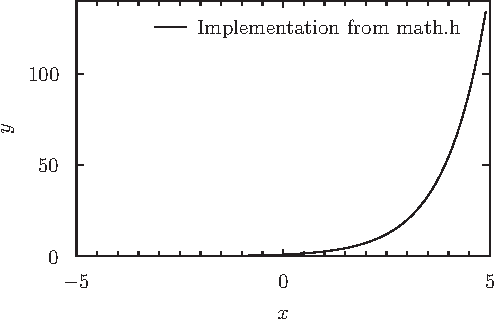
\includegraphics{true_exp_plot.pdf}
	\caption{A plot of the exponential function using 'exp' from math.h}
\end{figure}
This can be seen in figure \ref{fig:true}:

One of the most important properties of the exponential function is that it is it's own derivative. This is obvious from explicitly differentiating the series representation from equation \ref{eq:series}:

\begin{equation}
	\frac{\partial}{\partial x} e^{x} = \sum_{n=0}^{\infty} \frac{\partial}{\partial x} \frac{x^n}{n!}
	=
	\sum_{n=1}^{\infty} n \frac{x^{n-1}}{n!}
	=
	\sum_{n=1}^{\infty} \frac{x^{n-1}}{(n-1)!}
	=
	\sum_{n=0}^{\infty} \frac{x^n}{n!}=e^{x}
\end{equation}

\section{Numerical implementation}
The series representation is also convenient for numerical implementation, as integer powers are easily computed numerically. The natural choice of implementation would then look something like:

\begin{lstlisting}
double ex(double x){
return 1+x+pow(x,2)/2+pow(x,3)/3+pow(x,4)/4+pow(x,5)/5...
}
\end{lstlisting}

The dots represent not an infinite number of terms, but only a finite e.g. 10. However, this approach is bad for several reasons:
\begin{enumerate}
	\item We add terms off very different sizes since the sum is computed from left to right, resulting in large numerical error.
	\item We perform many operations! For each power of x, we use several multiplations.
	\item For large arguments, the convergence of the taylor expansion is not very good resulting in large errors.
	\item For negative arguments we add positive and negative terms, which is also very error prone. 

\end{enumerate}
Hence, a different approach is recommended:

		\begin{lstlisting}
double ex(double x){
if(x<0) return 1/ex(-x);
if(x> 1/.8) return pow(ex(x/2,2));
return 1+x*(1+x/2*(1+x/3*(1+x/4*(1+x/5*(1+x/6*(1+x/7*(1+...
}
		\end{lstlisting}

This solves all our problems: the sum is calculated from within, meaning that the smallest numbers are added first, the number of operations is reduced, large arguments are handled recursively so that the taylor expansion is only used for small arguments and negative arguments are computed using only strictly positive sums. 

\section{Test of our implementation}
To test our implementation, we plot results against the implementation from the standard C-library. The result can be seen isolated in figure \ref{fig:simple} and the comparison is found in figure \ref{fig:total}.

\begin{figure}\label{fig:simple}
	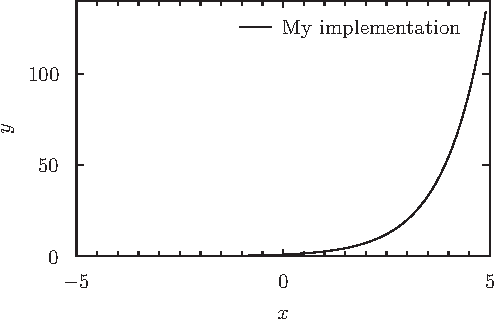
\includegraphics{simple_exp_plot.pdf}
	\caption{A plot of the exponential function using 'exp' from math.h}
\end{figure}

\begin{figure}\label{fig:total}
	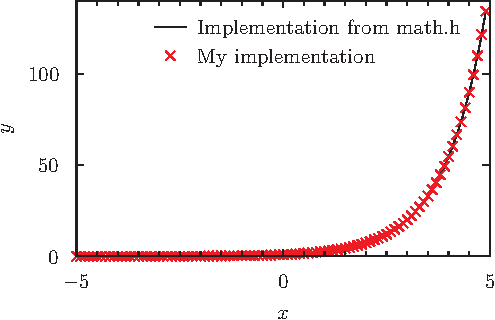
\includegraphics{total_exp_plot.pdf}
	\caption{A plot of the exponential function using 'exp' from math.h}
\end{figure}


\end{document}
